
%(BEGIN_QUESTION)
% Copyright 2008, Tony R. Kuphaldt, released under the Creative Commons Attribution License (v 1.0)
% This means you may do almost anything with this work of mine, so long as you give me proper credit

Suppose a set of three neon light bulbs were connected to a 3-phase alternator with the three stator winding sets labeled {\bf A}, {\bf B}, and {\bf C}:

$$\includegraphics[width=15.5cm]{i03257x01.eps}$$

The schematic diagram for this alternator/lamp system is as follows:

$$\includegraphics[width=15.5cm]{i03257x02.eps}$$

If the alternator spins fast enough (clockwise, as shown), the AC voltage induced in its windings will be enough to cause the neon lamps to ``blink'' on and off.  Most likely this blinking will be too fast to discern with the naked eye.

However, if we were to video-record the blinking and play back the recording at a slow speed, we should be able to see the sequence of light flashes.  Determine the apparent ``direction'' of the lamps' blinking (from right-to-left or from left-to-right), and relate that sequence to the voltage peaks of each alternator coil pair.

Furthermore, determine how to reverse the blinking sequence just by reconnecting wires between the alternator and the neon lamps.

\underbar{file i03257}
%(END_QUESTION)





%(BEGIN_ANSWER)

As the rotor spins clockwise, the lamps will blink from left to right ({\bf C}-{\bf B}-{\bf A}-{\bf C}-{\bf B}-{\bf A}).  To reverse the sequence, simply swap any two wires ($A \leftrightarrow B$, $B \leftrightarrow$ C, or $A \leftrightarrow C$).  Swapping any two phases will change a C-B-A sequence into an A-B-C sequence.

%(END_ANSWER)





%(BEGIN_NOTES)


%INDEX% Electronics review: 3-phase electrical power 

%(END_NOTES)


